% -*- mode:LaTeX; mode:visual-line; mode:flyspell; fill-column:75 -*-
\section{Results}
\label{sec:results}

We now present proof-of-concept experiments on a robot reaching task.
These early results serve as an initial demonstration of our ability to learn the correct behavior from user demonstrations and apply those when the user provides natural language command during execution.

The robot is tasked with reaching a goal, and the initial DS~($f^o(x)$) is a linear dynamics with a stable attractor at the goal position.

Using natural language, the user helps the robot reach the goal without hitting obstacles in a changing environment (note that the robot has no sensors to detect any obstacles).

\Cref{figBucket} shows one such scenario where the user can help the robot reach the goal (inside the bucket) by commanding it to ``come from above.''

Here the robot




Come from above
Come from below


\begin{figure}[t]
  \centering
  %% 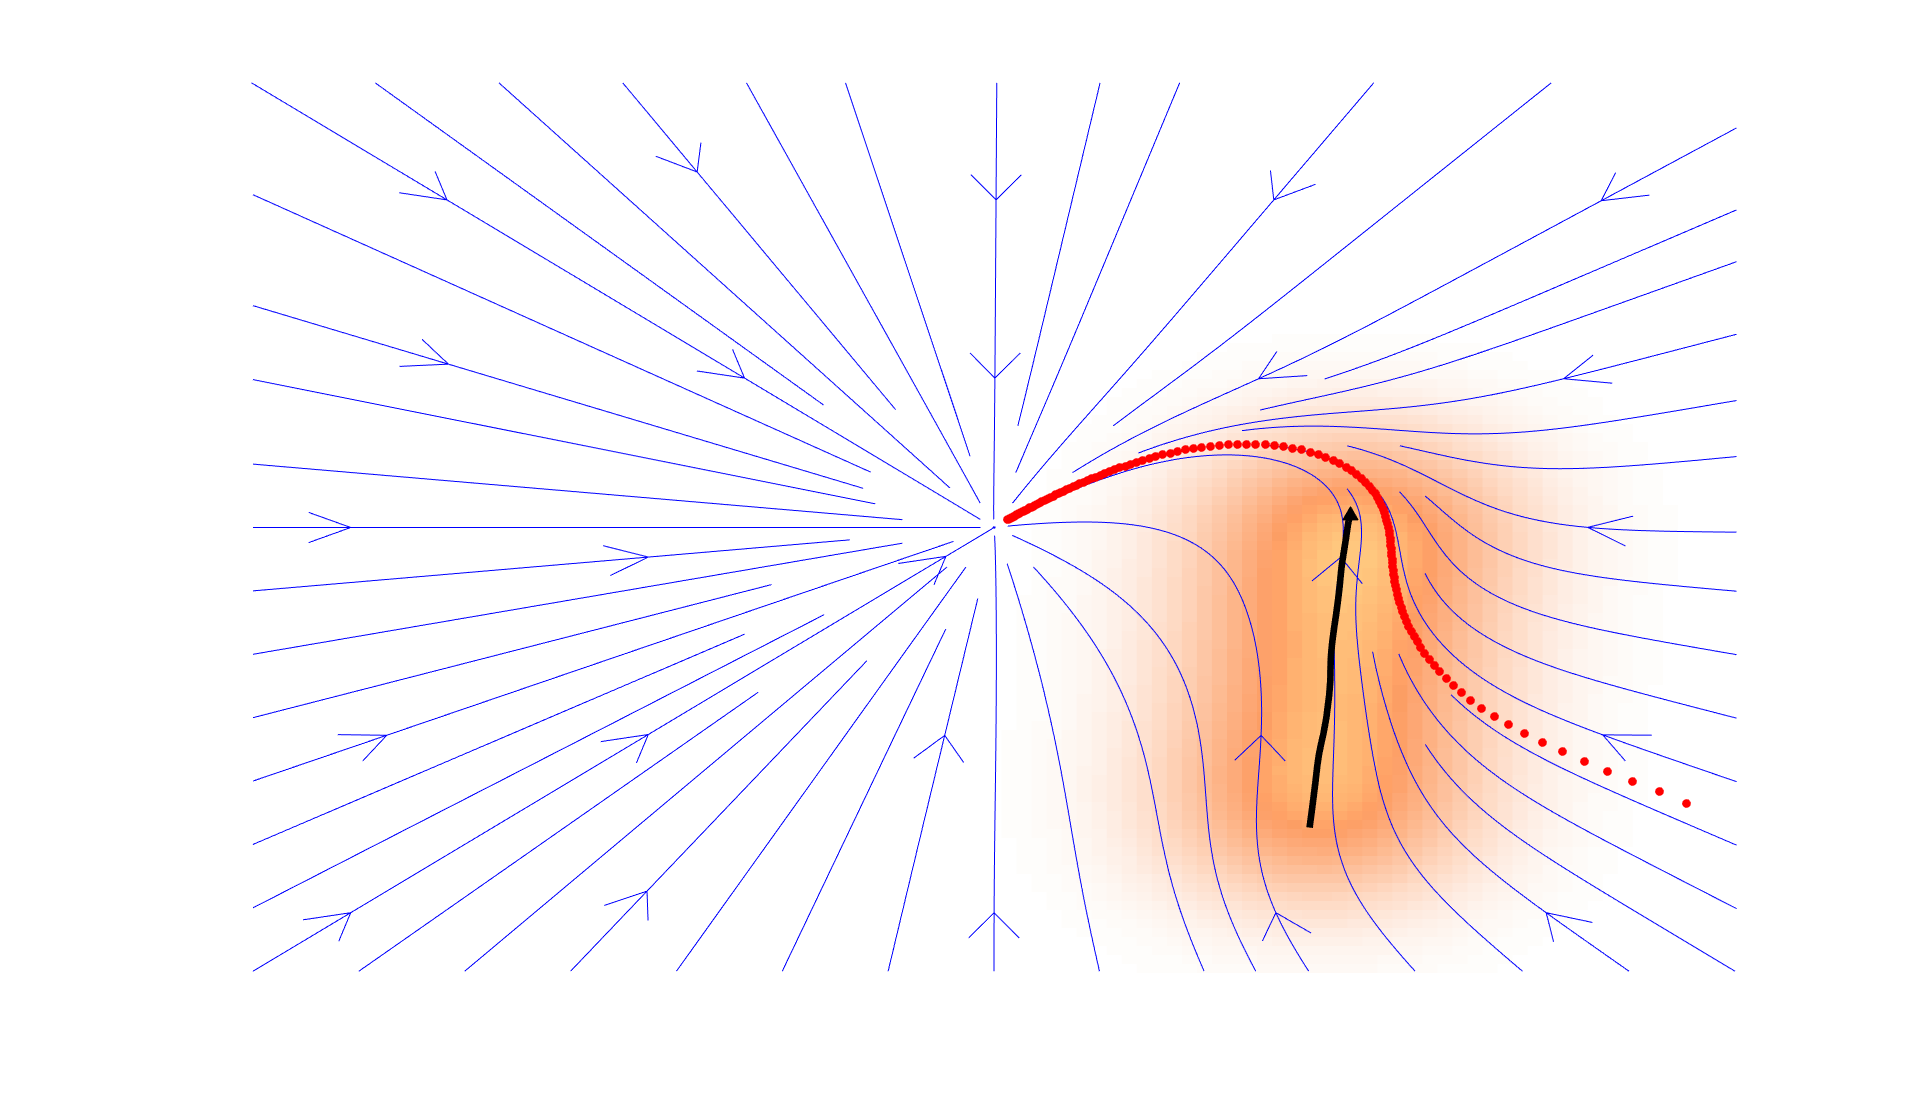
\includegraphics[
  %%   % trim = left bottom right top
  %%   trim = 150mm 50mm 100mm 80mm, clip,
  %%   width = 0.4\textwidth,
  %% ]{figs/gp_figs/3a-traj1.png}
  \missingfigure{Photo of the bucket}
  \caption{
    A scenario where the robot is unaware of the bucket and must get help from the user to reach the goal.
  }
  \label{figBucket}
\end{figure}
